% Preambel mit Einstellungen importieren
% Document type and used packages
\documentclass[open=right, % Kapitel darf nur auf rechten Seite beginnen
paper=A4,               % DIN-A4-Papier
a4paper,                % DIN-A4-Papier
11pt,                   % Schriftgöße
headings=small,         % Kleine Überschriften
headsepline=true,       % Trennlinie am Kopf der Seite
footsepline=false,      % Trennlinie am Fuß der Seite
bibliography=totoc,     % Literaturverzeichnis in das Inhaltsverzeichnis aufnehmen
twoside=off,            % Doppelseitiger Druck - auf off stellen für einseitig
DIV=7,
cleardoublepage=plain]{scrbook}

% Pakete einbinden, die benötigt werden
\usepackage[utf8]{inputenc}       % Dateien in UTF-8 benutzen
\usepackage[T1]{fontenc}          % Zeichenkodierung
\usepackage{graphicx}             % Bilder einbinden
\usepackage[ngerman]{babel}       % Deutsch unterstützen
\usepackage{xcolor}               % Color support
\usepackage{amsmath}              % Matheamtische Formeln
\usepackage{amsfonts}             % Mathematische Zeichensätze
\usepackage{amssymb}              % Mathematische Symbole
\usepackage{float}                % Fließende Objekte (Tabellen, Grafiken etc.)
\usepackage{booktabs}             % Korrekter Tabellensatz
\usepackage[printonlyused]{acronym}   % Abkürzungsverzeichnis [nur verwendete Abkürzugen]
\usepackage{makeidx}              % Sachregister
\usepackage{fancyhdr}             % Schönere Überschriften
\usepackage{listings}             % Source Code listings
\usepackage{listingsutf8}         % Listings in UTF8
\usepackage[hang,font={sf,footnotesize},labelfont={footnotesize,bf}]{caption} % Beschriftungen
\usepackage[scaled]{helvet}       % Schrift Helvetia laden
\usepackage[sf,bf,small]{titlesec} % Einstellungen für Überschriften
\usepackage[absolute]{textpos}	  % Absolute Textpositionen (für Deckblatt)
\usepackage{calc}                 % Berechnung von Positionen
\usepackage{blindtext}            % Blindtexte
\usepackage[bottom=40mm,left=35mm,right=35mm,top=30mm]{geometry} % Ränder ändern
\usepackage[backend=bibtex,style=verbose-trad2]{biblatex}
\usepackage{setspace}             % Abstände korrigieren
\usepackage{ifthen}               % Logische Bedingungen mit ifthenelse
\usepackage{scrhack}              % Get rid of tocbasic warnings
\usepackage[pagebackref=false]{hyperref}  % Hyperlinks
% \usepackage[all]{hypcap}          % Korrekte Verlinkung von Floats
\usepackage{pdflscape}            % Querformat für große Bilder
\usepackage[autostyle=true,german=quotes]{csquotes} % einheitliche Anführungszeichen
\usepackage{pifont}               %  Haken und Kreuze als Symbole bei der Nummerierung
\usepackage{graphics}
\usepackage{wrapfig}              % Grafiken umfließen den Text
\usepackage{caption}
\usepackage[listings,skins]{tcolorbox}

\bibliography{config/literatur.bib}   % BibTeX-Datei mit Literaturquellen einbinden

% Farben definieren
\definecolor{linkblue}{RGB}{0, 0, 100}
\definecolor{linkblack}{RGB}{0, 0, 0}
\definecolor{comment}{RGB}{63, 127, 95}
\definecolor{darkgreen}{RGB}{14, 144, 102}
\definecolor{darkblue}{RGB}{0,0,168}
\definecolor{darkred}{RGB}{128,0,0}
\definecolor{javadoccomment}{RGB}{0,0,240}

% Einstellungen für das Hyperlink-Paket
\hypersetup{
    colorlinks=true,      % Farbige links verwenden
%    allcolors=linkblue,
    linktoc=all,          % Links im Inhaltsverzeichnis
    linkcolor=linkblack,  % Querverweise
    citecolor=linkblack,  % Literaturangaben
	filecolor=linkblack,  % Dateilinks
	urlcolor	=linkblack    % URLs
}

% Einstellungen für Quelltexte
\lstset{
      xleftmargin=0.2cm,
      basicstyle=\footnotesize\ttfamily,
      keywordstyle=\color{darkgreen},
      identifierstyle=\color{darkblue},
      commentstyle=\color{comment},
      stringstyle=\color{darkred},
      tabsize=2,
      lineskip={2pt},
      columns=flexible,
      inputencoding=utf8,
      captionpos=b,
      breakautoindent=true,
	    breakindent=2em,
	    breaklines=true,
	    prebreak=,
	    postbreak=,
      numbers=left,
      numberstyle=\tiny,
      showspaces=false,      % Keine Leerzeichensymbole
      showtabs=false,        % Keine Tabsymbole
      showstringspaces=false,% Leerzeichen in Strings
      morecomment=[s][\color{javadoccomment}]{/**}{*/},
      literate={Ö}{{\"O}}1 {Ä}{{\"A}}1 {Ü}{{\"U}}1 {ß}{{\ss}}2 {ü}{{\"u}}1 {ä}{{\"a}}1 {ö}{{\"o}}1
}

\urlstyle{same}

% Einstellungen für Überschriften
\titlespacing{\paragraph}{0pt}{1ex}{2.0ex}
\titlespacing{\subsubsection}{0pt}{3ex}{0.0ex}
\titlespacing{\subsection}{0pt}{4ex}{0.2ex}
\titlespacing{\section}{0pt}{7ex}{1ex}
\titleformat*{\subsubsection}{\sffamily\itshape\bfseries\small}
\titleformat*{\paragraph}{\sffamily\bfseries\small}

% Einstellungen für Schriftarten
\setkomafont{pagehead}{\normalfont\sffamily}
\setkomafont{pagenumber}{\normalfont\sffamily}
\addtokomafont{footnote}{\footnotesize}

% Wichtige Abstände
\setlength{\parskip}{0.2cm}  % 2mm Abstand zwischen zwei Absätzen
\setlength{\parindent}{0mm}  % Absätze nicht einziehen
\clubpenalty = 10000         % Keine "Schusterjungen"
\widowpenalty = 10000        % Keine "Hurenkinder"
\displaywidowpenalty = 10000 % Keine "Hurenkinder"
\renewcommand{\footnotesize}{\fontsize{9}{10}\selectfont} % Größe der Fußnoten
\setlength{\footnotesep}{8pt} % Abstand zwischen den Fußnoten

% Index erzeugen
\makeindex

% Einfacher Font-Wechsel über dieses Makro
\newcommand{\changefont}[3]{
\fontfamily{#1} \fontseries{#2} \fontshape{#3} \selectfont}

% Eigenes Makro für Bilder
\newcommand{\bild}[5]{
\begin{figure}[htbp]
  \centering
  \includegraphics[width=#5\textwidth]{#1}
  \caption[#2]{#2\protect\footnotemark}
  \label{fig:#3}
\end{figure}
\footnotetext{#4}
}

\newcommand{\bildhochkant}[4]{
\begin{figure}[htbp]
  \centering
  \includegraphics[height=0.4\textheight]{#1}
  \caption[#2]{#2\protect\footnotemark}
  \label{fig:#3}
\end{figure}
\footnotetext{#4}
}

\newcommand{\bildquadrat}[4]{
\begin{figure}[htbp]
  \centering
  \includegraphics[width=0.560\textwidth,height=0.35\textheight]{#1}
  \caption[#2]{#2\protect\footnotemark}
  \label{fig:#3}
\end{figure}
\footnotetext{#4}
}

% Wo liegt der Sourcecode?
\newcommand{\srcloc}{src/}

\newcommand{\textitbf}[1]{\textit{\textbf{#1}}}

\lstset{basicstyle=\ttfamily,breaklines=true}
\newcommand{\shellcmd}[1]{\lstinline!\$#1!}

\newcommand{\sql}[1]{\lstinline[language=SQL]{#1}}

% Wo sind die Bilder?l
\graphicspath{{bilder/}}

% Makros für typographisch korrekte Abkürzungen
\newcommand{\zb}[0]{z.\,B.\ }
\newcommand{\dahe}[0]{d.\,h.\ }
\newcommand{\ua}[0]{u.\,a.\ }

%diverse Variablen um das Schreiben einfacher zu gestalten
\newcommand*{\fullref}[1]{\hyperref[{#1}]{\autoref*{#1} - \textit{\nameref*{#1}}}}

% format text like code
\newcommand{\code}[1]{\texttt{#1}}


% Dokumenteninfos importieren
% -------------------------------------------------------
% Daten für die Arbeit
% Wenn hier alles korrekt eingetragen wurde, wird das Titelblatt
% automatisch generiert. D.h. die Datei titelblatt.tex muss nicht mehr
% angepasst werden.

\newcommand{\srhsprache}{de} % de oder en für Deutsch oder Englisch

% Titel der Arbeit auf Deutsch
\newcommand{\srhtitel}{Data Engineering mit Apache Kafka}

% Weitere Informationen zur Arbeit
\newcommand{\srhort}{Mannheim}    % Ort
\newcommand{\srhautorvname}{Johannes} % Vorname(n)
\newcommand{\srhautornname}{Weber} % Nachname(n)
\newcommand{\srhautorzweivname}{Julian} % Vorname(n)
\newcommand{\srhautorzweinname}{Ruppel} % Nachname(n)
\newcommand{\srhmatnr}{11010021}
\newcommand{\srhmatnrzwei}{Matrikelnummer von Julian}
\newcommand{\srhdatum}{09.02.2018} % Datum der Abgabe
\newcommand{\srhjahr}{2018} % Jahr der Abgabe


\begin{document}
\frontmatter

% Römische Ziffern für die "Front-Matter"
\setcounter{page}{0}
\changefont{ptm}{m}{n}  %Times New Roman für den Fließtext
\renewcommand{\rmdefault}{ptm}

% Titelblatt
% -------------------------------------------------------
% In dieser Datei sollten eigentlich keine Veränderungen mehr
% notwendig sein.
% -------------------------------------------------------

\thispagestyle{empty}

% -------------------------------------------------------
\newcommand{\srhfakultaet}{Fakultät für Information, Medien und Design}%
\newcommand{\srhstudiengang}{Big Data und Business Analytics}%
\newcommand{\srhtyp}{Projektbericht}
\newcommand{\srhmaster}{Master of Science (M.Sc.)}
\newcommand{\srhkoerperschaft}{SRH Heidelberg}
\newcommand{\srhautorbib}{\srhautornname, \srhautorvname} % Autor Nachname, Vorname
\newcommand{\srhautor}{\srhautorvname \ \srhautornname} % Autor Vorname Nachname
\newcommand{\srhautorzwei}{\srhautorzweivname \ \srhautorzweinname} % Autor Vorname Nachname
\newcommand{\srhherbert}{Prof. Dr. Herbert Schuster} % Autor Vorname Nachname
\newcommand{\srhfrank}{Frank Schulz} % Autor Vorname Nachname
\newcommand{\srhbarbara}{Prof. Dr. Barbara Sprick}
\newcommand{\srhbianca}{Bianca Staffen}

% Daten in die Standard-Felder von KOMA-Script eintragen
\titlehead{\srhtyp\ in\  \srhstudiengang}
\subject{}
\title{\srhtitel}
\author{\srhauthor}
\date{\small{\srhdatum}}

% Daten für das fertige PDF-Dokument
\hypersetup{
  pdftitle={\srhtitel},  % Titel des Dokuments
  pdfauthor={\srhautor},              % Autor
  pdfsubject={\srhtyp\ in\ \srhstudiengang},                % Thema
  pdfkeywords={\srhtitel}         % Schlüsselworte
}

\newlength{\bindekorrektur}
\newlength{\seitenanfang}
\newlength{\seitenbreite}

\setlength{\bindekorrektur}{-46mm}   % Korrektur der horizontalen Position
\setlength{\seitenanfang}{0mm}       % Korrektur der vertikalen Position
\setlength{\seitenbreite}{297mm}

\begin{figure}[h]
  \flushright
  
\includegraphics[width=7cm]{srh_logo.png}
\end{figure}


% Titel der Arbeit
\begin{textblock*}{\seitenbreite}(\bindekorrektur,\seitenanfang + 62mm) % 4,5cm vom linken Rand und 6,0cm vom oberen Rand
  \centering\Large\sffamily
  \vspace{4mm} % Kleiner zusätzlicher Abstand oben für bessere Optik
  \textbf{\srhtitel}
\end{textblock*}%

% Projektbericht
\begin{textblock*}{\seitenbreite}(\bindekorrektur,\seitenanfang + 103mm)
  \centering\large\sffamily
  \srhtyp
  \vspace{2mm} \\
  von
\end{textblock*}

% Name
\begin{textblock*}{\seitenbreite}(\bindekorrektur,\seitenanfang + 130mm)
  \centering\large
  \textbf{\srhautor} \\
  \vspace{2mm}
  Matrikelnummer: \srhmatnr \\
  \vspace{5mm}
  und
\end{textblock*}

% Name 2
\begin{textblock*}{\seitenbreite}(\bindekorrektur,\seitenanfang + 155mm)
  \centering\large
  \textbf{\srhautorzwei} \\
  \vspace{2mm}
  Matrikelnummer: \srhmatnrzwei
\end{textblock*}

% Datum
\begin{textblock*}{\seitenbreite}(\bindekorrektur,\seitenanfang + 185mm)
  \centering\large
  \textsf{\srhdatum}
\end{textblock*}

% Fakultät
\begin{textblock*}{\seitenbreite}(\bindekorrektur,\seitenanfang + 205mm)
  \centering\large\sffamily
  \srhkoerperschaft \\
  \vspace{2mm}
  \srhfakultaet \\
  \vspace{2mm}
  \srhstudiengang
\end{textblock*}

% Dozent(en)
\begin{textblock*}{\seitenbreite}(\bindekorrektur,\seitenanfang + 250mm)
  \centering\large\sffamily
  Dozent \\
  \vspace{2mm}
  \srhfrank
\end{textblock*}

% Bibliographische Informationen
\null\newpage
\thispagestyle{empty}

\newcommand{\srhbib}{\begin{small}\textbf{\srhautorbib}: \\ \srhtitel \ / \srhautor. \ -- \\ \srhtyp, \srhort \: \srhkoerperschaft, \srhjahr. \pageref{lastpage} Seiten.\end{small}}


% Inhaltsverzeichnis erzeugen
\phantomsection
\tableofcontents

% Korrigiert Nummerierung bei mehrseitigem Inhaltsverzeichnis
\cleardoublepage
\newcounter{frontmatterpage}
\setcounter{frontmatterpage}{\value{page}}

% Arabische Zahlen für den Hauptteil
\mainmatter

% Den Hauptteil mit vergrößertem Zeilenabstand setzen
\onehalfspacing

% ------------------------------------------------------------------
% Hauptteil der Arbeit
\chapter{Einleitung}
\label{chap:einleitung}

\section{Aufgabe und Ziel}
Im Rahmen dieses Projektes war es die Zielstellung sich mit Data Ingestion, Data Storage sowie Data Retrieval vertraut zu machen.
\paragraph{Data Ingestion} ist die Beschaffung der Daten.
Dies kann entweder mit Hilfe eines Data Streams erfolgen oder einer statischen Datenquelle - also eine Datei die lokal
auf einem Rechner abgelegt wird wie \zb{} eine \ac{CSV} oder \ac{JSON} Datei.

Unter einem Data Stream versteht man einen kontinuierlichen Datenstrom wie \zb{}
die Erstellung von immer wieder neuen Twitter Nachrichten.\\
Ein wichtiges Merkmal eines Data Streams ist, dass nicht vorherzusehen ist wann der Datenstom zu Ende ist - er könnte theoretisch unendlich sein.
\\
Im Falle des Twitter Datenstroms ist es nicht abzusehen wann die letzte Twitter Nachricht geschrieben wird.

Für unsere Aufgabe ist darauf zu achten, dass der Datenstrom über ein \ac{API} öffentlich zugänglich.

\paragraph{Data Storage} ist die Speicherung der Daten.
Hierbei wurde uns die Anforderung gestellt, das für die Speicherung der Daten die Streaming Plattform Apache Kafka verwende wird.
Des Weiteren war es gestattet die Daten zusätzlich in einer relationen Datenbank, NoSQL Datenbank oder mit Spark Streaming zu speichern.

\paragraph{Data Retrieval} ist die Beschaffung der Daten aus einer Datenbank mit \ac{SQL} Abfragen und die abschließende Ausgabe
der Ergebnisse in Form von Tabellen oder einfachen Visualisierungen. \\
Es sollen mindestens drei verschieden \ac{SQL} Abfragen abgesetzt werden mit unterschiedlichen Filter- und Agreggatsfunktionen sowie einer Teilaggregation wie \zb{} GROUP BY.
\\
Die Visualisierung der Daten soll in einem virtuellen Notebook erfolgen.
\\
Als virtuelles Notebook durften wir zwischen Apache Zeppelin oder Jupyter entscheiden.

Unsere Aufgabe ist es eine geeignete Vorgehensweise für die Bewältigung dieser Aufgabe zu finden und umzusetzen.

Wir entschieden uns für unser Szenario Daten von NYC Open Data zu nutzen.\\
NYC Open Data gibt allen \glqq New Yorkern\grqq{} und somit auch der ganzen Welt, die Chance, Open Data, also frei zugängliche Daten,
einfach zu konsumieren.\autocite{NYCOpenData}

NYC Open Data ermöglicht es sowohl einen kontinuierlichen Data Stream als auch eine statische \ac{CSV} Datei zu konsumieren.
Dank diesem Umstand entschieden wir uns im Rahmen dieses Projektes beide Möglichkeiten umzusetzen und zu vergleichen.
Auch bei Data Retrieval entschieden wir uns dafür sowohl Apache Zeppelin als auch Jupyter zu nutzen und zu vergleichen.

\fullref{chap:tools} beschäftigt sich detailierter mit den verwendeten Tools und Programmiersprachen.

\fullref{chap:loesung} erläutert das gewählte Szenario und die verwendeten Architektur sowie die Lösung zu den Themen Data Ingestion, Data Storage und Data Retrieval.

\chapter{Werkzeuge und technische Rahmenbedingungen}
\label{chap:tools}
Im folgenden Abschnitt werden einige wichtige technische Werkzeuge, die im späteren Verlauf eingesetzt werden, kurz und prägnant erläutert.
\begin{figure}[h]
	\centering
	
\includegraphics[width=7cm]{logos.pdf}
	\label{fig:logos}
\end{figure}

\begin{description}
	\item [Java] ist eine objektorientierte Open-Source Programmiersprache die ursprünglich von Sun Microsystems entwickelt wurde und heute zum Oracle Konzern gehört. In den letzten beiden Hauptversionen wurde der Sprachumfang  um funktionale und reaktive Aspekte erweitert. Java ist dank der \textit{Java Virtual Maschine} (JVM) als Laufzeitumgebung plattformunabhängig und hat sich vorwiegend in Enterprise Systemen und Web-Backends etabliert. Im Zuge der Verbreitung von BigData Projekten unter dem Dach der Apache Software Foundation, allem voran Hadoop und Spark, werden JVM sprachen wie Java und Scala nun auch im Bereich BigData eingesetzt.
	\item [Python] ist eine Open-Source Skripsprache, die sich hauptsächlich durch eine gut lesbare und knappe Syntax auszeichnet und unter anderem das objektorientierte und funktionale Programmierparadigma unterstützt. Im Gegensatz zu Java ist Python dynamisch typisiert und wird interpretiert anstatt kompiliert. Dank eines sehr umfangreichen und ausgereiften Ökosystems aus Frameworks und Bibliotheken zur Datenanalyse und maschinelles Lernen\footnote{z.B. TensorFlow von Google} ist Python im Bereich BigData  und dank der minimalinvasiven Eigenschaften zum Rapid Prototyping beliebt.
	\item [Apache Kafka] ist eine verteilte Data-Streaming Plattform der Apache Software Foundation, die ursprünglich von LinkedIn entworfen wurde. Beliebt ist Kafka im BigData Umfeld wegen seiner Skalierbarkeit und Fehlertoleranz.  Zu den Einsatzszenarien zählen vor allem Stream Processing, es kann aber auch als reiner Message Broker oder Speichersystem für Streaming Data verwendet werden. Die wesentlichen Komponenten von Kafka sind \textbf{\textit{Producer}} um einen Stream für einen \textbf{\textit{Topic}} zu veröffentlichen, \textbf{\textit{Kafka Cluster}} um die die Streaming-Daten verteilt pro \textit{Topic} im Dateisystem zu speichern und \textbf{\textit{Consumer}} um einen \textit{Topic} zu abonnieren und dessen Nachrichten zu lesen. Zudem können mit \textbf{\textit{Kafka Streams}} Nachrichten im Cluster transformiert werden. Mittels \textbf{\textit{Kafka Connectors}} kann man per Konfiguration gängige Datenquellen und -senken\footnote{wie z.B. Twitter oder JDBC} anschließen und stellen somit eine deklarative alternative zu den imperativen \textit{Producer API} und \textit{Consumer API} dar.
	2014 haben sich die verantwortlichen LinkedIn Mitarbeiter vom Mutterkonzern getrennt um sich mit der neu gegründeten Firma Confluent dediziert dem Apache Kafka Ökosystem zu widmen. Entwickelt wurde die quelloffene Software in der JVM-basierten Programmiersprache Scala, welche objektorientierte und funktionale Aspekte vereint.
	\begin{figure}[h]
		\centering
		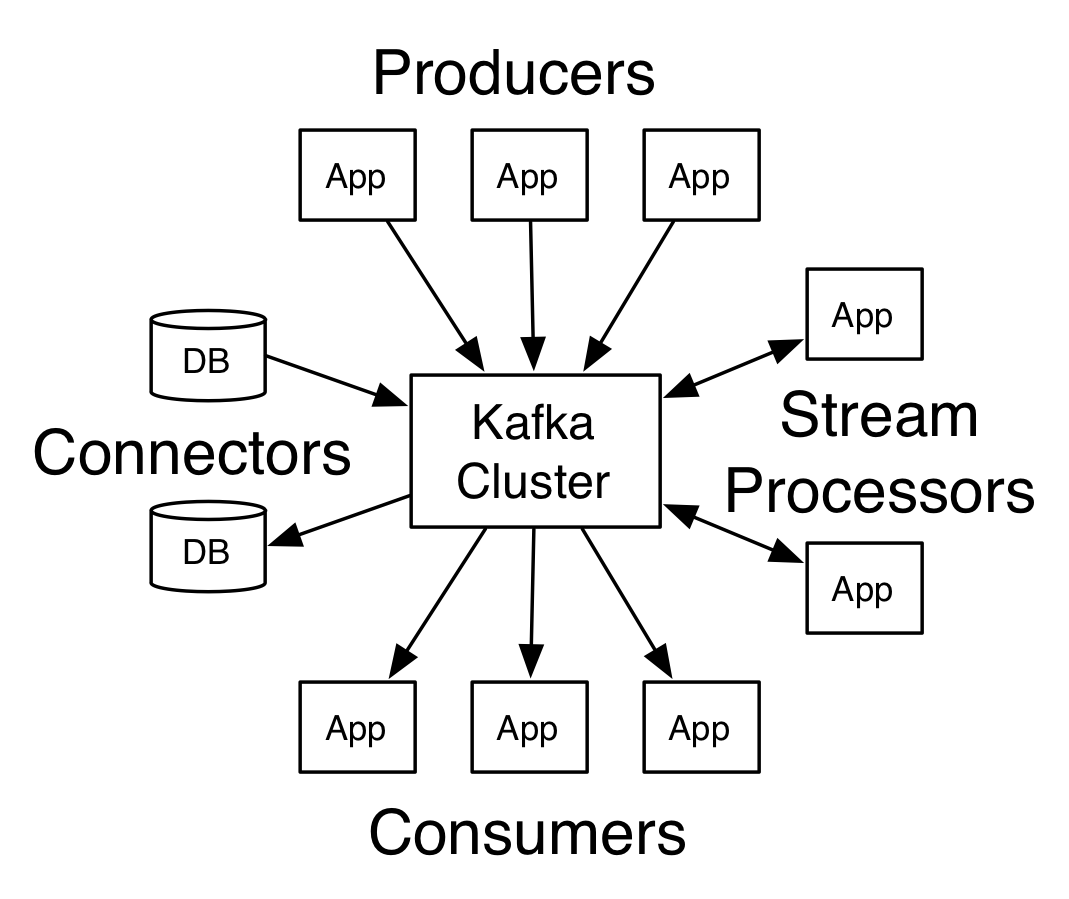
\includegraphics[width=7cm]{kafka-apis.png}
		\caption[Apache Kafka Architektur]{Apache Kafka Architektur\autocite{TODO}}
		\label{fig:KafkaArchitecture}
	\end{figure}
	\item [PostgreSQL] ist ein objektrelationales Datenbankmanagementsystem. Das vollständig ACID-konforme und in C geschriebene quelloffene System zeichnet sich durch einen breiten Funktionsumfang, Stabilität, Standardkonformität, hohe Erweiterbarkeit, und als Resultat dessen, eine weite Verbreitung aus. Neben dem traditionellen zeilenorientierten  Eigenschaften bietet PostgreSQL zudem Erweiterungen hinsichtlich verteilter, hoch-parallelisierter und  spaltenorientierter Datenverarbeitung, ein Geoinformationssystem sowie Volltextsuche. Auch im Bereich NoSQL bietet PostgreSQL eine dokumentenorientierter Speicherung und durch Erweiterungen sogar Graphen und Schlüssel-Werte-Datenstrukturen. Diese Flexibilität eröffnet PostgreSQL vielseitige Einsatzszenarien, darunter sowohl OLTP als auch OLAP.
	\item [Apache Zeppelin] ist eine Web-basierte Open-Source Software mit der man sog. Notebooks zur datengetriebenen, interaktiven und kollaborativen Analyse erstellen kann. Es werden eine Vielzahl an Speicher- und Analysetechnologien unterstützt, darunter SQL, Scala, Spark, Python und R. Im wesentlichen werden in einem Notebook polyglotte Abfrageskripte ad-hoc gegen die diversen Datenquellen ausgeführt und deren Ergebnisse in einem AngularJS, konfigurierbaren Web-Dashboard visuell und interaktiv dargestellt. Dadurch eignet es sich sowohl zur explorativen Datenanalyse als auch zum veröffentlichen und teilen von Analyseergebnissen.
	\item [Jupyter] ähnelt in den meisten Aspekten Apache Zeppelin, sodass sich alle oben zu Zeppelin genannten Punkte auch zu Jupyter nennen lassen. Die Unterschiede liegen eher im Detail der einzelnen Funktionen sowie der historisch und organisatorisch bedingten Nähe zu bestimmten Schlüsseltechnologien. Für das hier behandelte Forschungsprojekt spielen die individuellen Stärken und Schwächen der beiden Werkzeuge jedoch keine Rolle, weshalb beide Werkzeuge ebenbürtig eingesetzt werden.
	\item[\ac{SODA}] ist eine quelloffene Open Data Web-Programmierschnittstelle des U.S. Amerikanischen Dienstleisters Socrata. Anhand URLs werden Datasets adressiert und mittels der an SQL angelehnten \textit{Socrata Query Language} (SoQL) per HTTP GET in unterschiedlichen Datenformaten abgefragt. Zudem stehen SDKs für diverse Programmiersprachen zur Verfügung. Im Rahmen des Projektes werden wir die Datensätze der \ac{API} im \ac{JSON} Dateiformat abrufen.
	\begin{figure}[h]
		\centering
		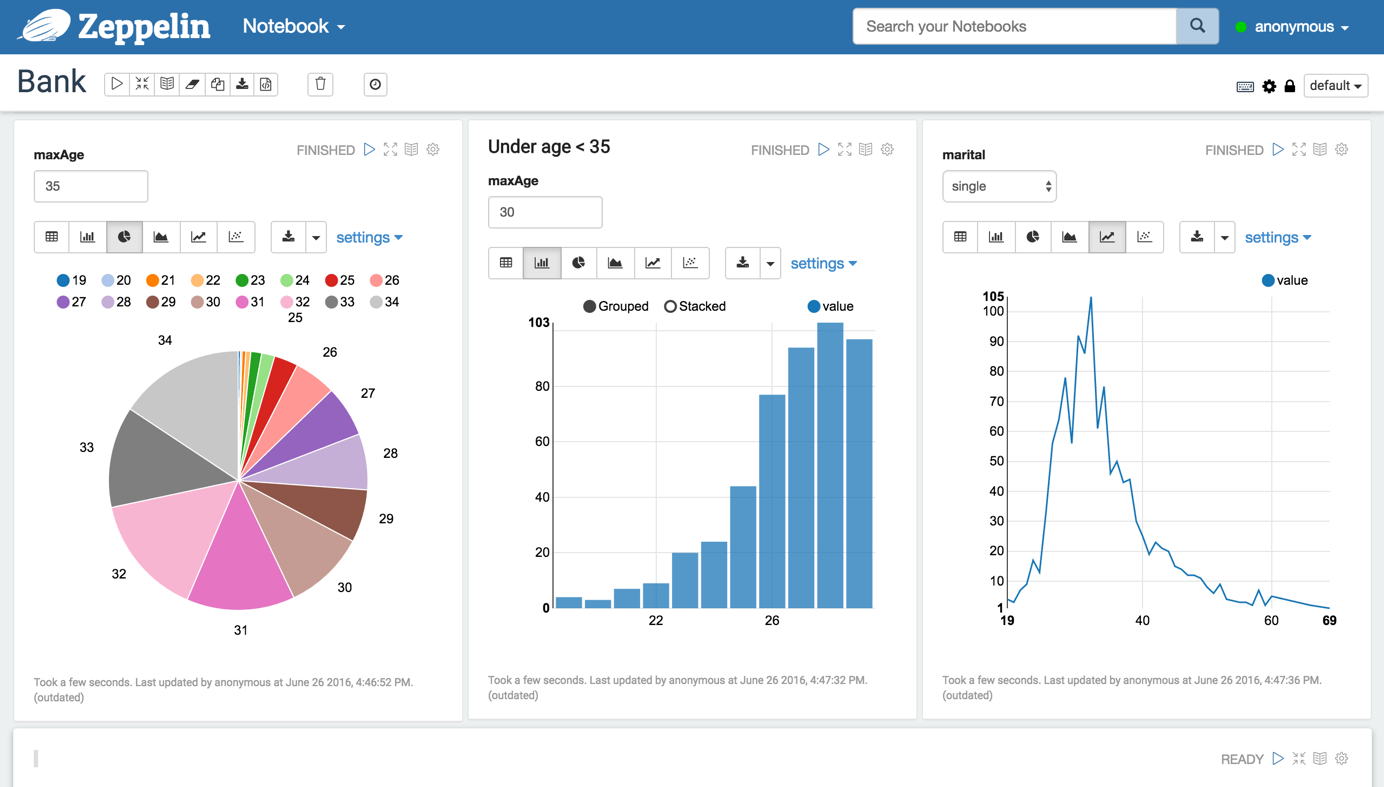
\includegraphics[width=\linewidth]{zeppeln_example_notebook.png}
		\caption[Beispielhaftes Notebook mit Apache Zeppelin]{Beispielhaftes Notebook mit Apache Zeppelin\citep{TODO}}% https://zeppelin.apache.org/assets/themes/zeppelin/img/notebook.png
		\label{fig:zeppeln_example_notebook}
	\end{figure}
\end{description}

\chapter{Lösungsansatz}
\label{chap:loesung}

In diesem Kapitel wird ein Konzept und Herangehensweise zur Lösung der in 1TODO genannten Problemstellung erörtert.

\section{Architekturentscheidungen}

Lambda vs. Kappa

Warum Lambda?
stream ist unendlich. Ergebnisse/Aggregationen zwischenspeichern
Aggregationen mit den Live Daten abmischen!
Nachteile googlen
Quelle verweisen

Warum Kappa?
Daten sind endlich aber ausreichend für unsere Bedürfnisse.
Haben eh nur Pseudostream.
Vorteile googeln

https://www.confluent.io/blog/simplest-useful-kafka-connect-data-pipeline-world-thereabouts-part-1/
Grafik einbetten

\section{Data Ingestion}

Wie in \fullref{chap:einleitung} erläutert wird für die Erstellung des Prototyps NYC Open Data als Datenquelle genutzt.

NYC Open Data bietet verschiedene Datenätze an um an die unterschiedlichsten Informationen aus New York zu gelangen
wie \zb{} der Standort von öffentlichen Wi-Fi Hotspopts oder offene Stellenauschreibungen.\autocite{NYCOpenDataExample}

Innerhalb dieses Projektes wird der Datensatz mit dem Kürzel \textit{fhrw-4uyv} verwendet.
Er beinhält alle Service Request die seit 2011 von den Einwohner von New York City abgesetzt worden sind.

Beispielsweise kann mit diesem Datensatz herausgefunden werden wo welche Straßenlaternen in New York City ausgefallen sind
oder in welchem Haus zu welcher Uhrzeit gefeiert wurde da sich jemand über den Lärm beschwert hat.

In unserem Projekt beschaffen wir die Daten über eine \ac{CSV} Datei die man sich bei NYC Open Data herunterladen kann
und direkt über die \ac{SODA} \ac{API} die einen eigenen Endpunkt anbietet um die Service Requests abzufragen.

Die Data Ingestion per \ac{CSV} Datei setzte Julian Ruppel mit der Programmiersprache Java um und
den kontinuierlichen Datenstrom über die \ac{SODA} \ac{API} wurde von Johannes Weber mit der Programmiersprache Python
ausgelesen.

Beide Ansätze werden in diesem Kapitel beschrieben und anschließend miteinander verglichen.

\subsection{Data Ingestion via \acs{SODA} Schnittstelle}
Wie in \fullref{sec:arch} erläutert ist es die Aufgabe des Data Ingestion Prototyps zum einen Daten aus der externen Quelle auszulesen
aber auch die Daten direkt an die Apache Kafka Plattform weiterzuleiten und in ein Topic zu speichern.

Die Umsetzung des "Producers" erfolgte mit Python.
Zusätzlich wurden folgende Frameworks benutzt um die Implementierung des \textit{producers} zu unterstützen:

\begin{itemize}
  \item sodapy
  \item kafka-python
\end{itemize}

Sobald der \textit{producer} ausgeführt wird, wird der Nutzer gebeten ein Anfangs- und Enddatum anzugeben.
In diesem Zeitfenster werden dann alle Datensätze abgefragt und in das Topic "ServiceRequests" von Apache Kafka geschrieben.

\subsubsection{Quellcode}
Der \textit{producer} besteht insgesamt aus zwei Python Skripten:

\begin{itemize}
  \item SodaHelper.py
  \item producer.py
\end{itemize}

Das SodaHelper Skript ist ein separatzer Wrapper um die sodapy Bibliothek um die Verbindung zu der API herzustellen und die Daten zu holen.
Somit wird eine klare Aufgabentrennung erreicht.
Das Skript SodaHelper ist für die Verbindung zu der API zuständig und das producer Skript nur für die Weiterleitung der empfangenen Daten an Apache Kafka.

Da es sich hierbei nicht um ein Live Stream handelt wie \zb{} bei Twitter API, haben wir uns dazu entschieden einen "Fake Stream" zu erstellen,
indem nicht alle Daten sofort an Apache Kafka weitergeleitet werden sondern immer ein gewisser Abstand zwischen dem Senden der einzelnen Datensätze
erzwungen wird.

Unser ausgewählter Datensatz ist sehr groß. Wenn \zb{} der Nutzer Daten von einem Monat abrufen will kann es vorkommen, dass in diesem Zeitraum mehr als 100.000 Datensätze
bereit zum Abruf stehen.
Da der Abruf von einer solch großen Menge an Daten über die API eine sehr hohe Rechenleistung erfordert und diese im Rahmen des Projektes nicht zur Verfügung steht wurde
eine Art \textit{Paging} entwickelt.
Durch die feste Angabe eines Limits von 10.000 wird sichergestellt, dass ein Request an die \ac{SODA} \ac{API} nur maximal 10.000
Datensätze liefern kann und durch einen entwickelten Algorithmus werden so lange Requests ausgeführt bis der gewünschte Zeitraum des Users komplett empfangen und
die Request an Apache Kafka gesendet wurden.

Vorgegeben durch das Framework \textit{kafka-python} können die Einträge eines Topics nur als byte String abgelegt werden.
Aus diesem Grund wird der empfangende Datensatz zuerst in ein byte string umgewandelt bevor er an Apache Kafka gesendet wird.

Folgendes Code Snippet zeigt den entwickelten Algorithmus um das Paging zu realisieren.
Mit Hilfe des SodaHelpers werden zunächst die Datensätze von der API - unter Berücksichtigung des Limits, des Anfangs- und Enddatums geholt.
Wie in dem Snippet zu erkennen wird die Variable \textit{limit} in dem Skript gesetzt.
die Variablen \textit{from\_date} und \textit{to\_date} werden beim Starten des Skripts von dem User gesetzt.

Der Algorithmus beruht auf der Annahme, dass wenn der empfangene Datensatz genau die Länge des Limits hat es immer noch weitere Datensätze gibt die von der API abgerufen werden müssen.
Wenn also das Limit erreicht wurde wird das Datum des letzten Datensatzes als neues Enddatum festgelegt und der Prozess beginnt von vorne, solange die Anzahl der empfanenen Datensätze nicht mehr dem Limit entsprechen
oder die verwendeten Anfangs- und Enddatumswerte identisch sind.

\lstinputlisting[language=Python, firstline=20, lastline=45]{../python/producer.py}

\subsection{Data Ingestion via CSV Datei}\label{subsec:csv}
Als offline-fähige Alternative zur \ac{SODA} API gibt es einen weiteren Kafka Producer in Java.
Dieser liest die Nachrichten zeilenweise aus einer lokalen \ac{CSV} Datei ein und publiziert die Datensätze als \ac{JSON} einzeln an einen Kafka Topic.
Die \ac{CSV} Datei wurde vorher aus dem NYC OpenData Portal runtergeladen.

Der Programmablauf lässt sich in wenigen Stichpunkten beschreiben:
\begin{enumerate}
	\item Verbindung des \code{KafkaProducer<Long, String>} zum Kafka Cluster konfigurieren.Dazu zählen hauptsächlich Host und Port sowie die Datentypen, um Schlüssel und Wert der Nachrichten zu serialisieren.
	\item Zeilenweises einlesen der \ac{CSV} Datei und dabei jeweils den Datensatz in einen \ac{JSON}-String transformieren, diesen \code{String} als Wert in einen \code{ProducerRecord<Long, String>} setzen und an den bestimmten Kafka Topic senden. Um einen realen Stream zu simulieren wartet der Producer-Thread pro verarbeiteten Datensatz eine zufällige Wartezeit zwischen 0 bis 2 Sekunden.
\end{enumerate}

Listing \ref{listing:javacsvproducer} zeigt einen Überblick über die relevanten Methoden.

%\begin{tcblisting}{width=19cm,listing only,blank,tikz={rotate=90},listing options={basicstyle=\ttfamily}}
\lstinputlisting[language=Java, firstline=37, lastline=68, label=listing:javacsvproducer,
	captionpos=b,
	caption=Auszug aus \code{com.srh.bdba.dataengineering.MyProducer}]{../java/src/main/java/com/srh/bdba/dataengineering/MyProducer.java}
%\end{tcblisting}

Zur Implementierung wurden folgende Bibliotheken über Maven eingebunden:
\begin{itemize}
	\item \code{org.apache.kafka:kafka-clients}
	\item \code{org.apache.commons:commons-csv}
	\item \code{com.fasterxml.jackson.core:jackson-core}
	\item \code{com.fasterxml.jackson.core:jackson-databind}
\end{itemize}


\section{Data Storage}
Apache Kafka wird dazu verwendet um den kompletten Datensatz eines Service Requests abzuspeichern.
Ein Consumer liest die Daten von Apache Kafka aus und speichert die relevanten Attribute eines Datensatzes in der Datenbank.
Als Datenksystem haben wir in unserem Projekt für PostgreSQL entschieden.

Zunächst erstellten wir eine Tabelle mit dem Namen \textitbf{service\_request} um die Service Requests von New York zu speichern.
Eine stichprobenartige Analyse des Datensatzes hat ergeben, dass einzelne Felder des original Datensatzes sehr häufig mit \code{NULL}
Werten belegt sind.
In der Datenbanktabelle \textitbf{service\_request} wurden diese Felder außer Acht gelassen.

Die Datenbanktabelle besitzt folgende Attribute
\begin{enumerate}
  \item unique\_key
  \item created\_date
  \item agency\_name
  \item complaint\_type
  \item descriptor
  \item longitude
  \item latitude
  \item agency
  \item location\_type
  \item incident\_zip
  \item incident\_address
  \item street\_name
  \item cross\_street\_1
  \item cross\_street\_2
  \item address\_type
  \item city
  \item status
  \item due\_date
  \item borough
  \item resolution\_description
\end{enumerate}

In der offiziellen Dokumentation des Datensatzes werden die einzelnen Attribute
eines Service Requests genau beschrieben und deren technische Bezeichner aufgelistet.
\footnote{https://dev.socrata.com/foundry/data.cityofnewyork.us/fhrw-4uyv}

Die Attribute der Tabelle \textitbf{service\_request} sind identisch zu den
Bezeichnern des original \ac{SODA} Datensatzes.

Um das Handling mit Aoache Kafka zu vereinfachen wurden zwei weitere Python
Bibliotheken installiert.
Diese sind:

\begin{itemize}
  \item kafka-python
  \item sqlalchemy
  \item psycopg2 (wird von sqlalchemy benötigt)
\end{itemize}

Genau wie bei dem Producer abstrahiert das Paket \code{kafka-python} die Verbindung zu unserem Apache Kafka Server und erleichtert den Zugriff auf das Topic.
Durch den Einsatz von \code{sqlalchemy} ist es möglich auf die Datenbank und deren Tabelle(n) in einer objektorientierten Weise zuzugreifen
und die Ausführung von \ac{SQL} Statements wird vereinfacht bzw. durch Klassenmethoden abstrahiert.

\subsubsection{Python Quellcode Programmablauf}
\label{subsub:quellcode_storage}
Neben den verwendeten Bibliotheken besteht derConsumer aus zwei Python Skripten.

\begin{itemize}
  \item DBHelper.py
  \item consumer.py
\end{itemize}

Während sich das \code{consumer} Skript um das Auslesen eines Kafka Topics kümmert ist die \code{DBHelper} Klasse
für die Verbindung zu der Datenbank zuständig, liest Tabellenspalten aus und speichert einen Datensatz in der Tabelle.

Nachfolgend die Code Snippet der Consumer Klasse.

\lstinputlisting[language=Python, firstline=13, lastline=27]{../python/Consumer.py}

Sobald das Consumer Skript aufgerufen wird, wird eine Verbindung mit der Datenbank
aufgebaut und der \code{KafkaConsumer} stellt eine Verbindung mit dem Apache Kafka
Server bzw. dem Topic "ServiceRequest" her.
(Zeile 1 - 9)

Sobald von seitens des Producers ein neuer Datensatz in das Topic "ServiceRequests" geschrieben wird,
wird der Datensatz ausgelesen in ein \ac{JSON} umgewandelt, die benötigten Attribute aus dem \ac{JSON} gelesen
und in ein temporäres Dictionary geschrieben.
Dieses Dictionary wird abschließend mit Hilfe des \code{DBHelper} Skripts in die
Datenbanktabelle geladen.
(Zeile 11 - 18)

Wie eingangs erwähnt bezeichneten wir die Attribute der Datenbanktabelle und des \ac{SODA} Datensatzes identisch.

Mit diesem kleinen \glqq Kniff\grqq{} kann mit Hilfe der Namen der Tabellenspalten
auf die Keys des \ac{JSON} zugegriffen, den zugehörigen Wert ausgelesen und als neuen Wert für das temporäre Dictionary genutzt werden.
(Zeile 14 - 16)

\subsubsection{Java Quellcode Programmablauf}
Auch für den Consumer gibt es eine alternative Implementierung in Java.
Diese findet sich in \code{com.srh.bdba.dataengineering.MyConsumer}.
Der Programmablauf ist ähnlich zu der Python Implementierung, weshalb an dieser Stelle auf Codelistings im Anhang TODO verwiesen wird.
Kurz zusammengefasst wird ein \code{KafkaConsumer<Long, String>} konfiguriert und pro 100 Millisekunden am Kafka-Cluster nachgefragt, ob es neue \code{ConsumerRecord <Long, String>} für das entsprechende Topic gibt.
Falls dem so ist wird die \ac{JSON} Nachricht aus dem \code{ConsumerRecord<Long, String>} ausgepackt und per \code{PreparedStatement} über \code{JDBC} in die PostgreSQL Tabelle eingefügt.

\section{Data Retrieval}
Die Aufgabe im Bereich Data Retrieval war es die zum einen die Daten aus der Datenbank auszulesen und diese mit einem virtuellen Notebook zu visualisieren.

Die Beschaffung und Auswertung der Daten mit Apache Zeppelin übernahm Julian Ruppel.
Johannes Weber bereitete die Daten mit Python auf und visualisierte sie in einem Jupyter Notebook.
\subsection{Data Retrieval mit Apache Zeppelin}
Apache Zeppelin bringt standardmäßig einige nützliche Funktionen mit, die es für die Datenauswertung interessant machen. Dazu zählen u.A.:
\begin{itemize}
	\item SQL via JDBC inkl. PostgreSQL Support
	\item Interaktive Diagramme über Formulargeneriung und Pivot-Charts
	\item Frei konfigurierbare Anordnung der Diagramme im Notebook
	\item Versionsverwaltung für Notebooks um verschiedene Stände abzuspeichern und schnell zwischen Versionen zu wechseln
\end{itemize}

Über den Befehl \shellcmd{/bin/zeppelin.sh} startet Zeppelin und ist standardmäßig im Browser über den Port 8080 erreichbar. Die gesamte Konfiguration, Entwicklung und Ausführung des Notebooks erfolgt im Web. Letztlich ist ein Notebook ein Kanvas in den man Kacheln erstellen und verwalten kann. Jede Kachel besteht aus 3 integralen Bestandteilen:
\begin{itemize}
	\item \textbf{Code} der mittels der vielen Interpreter die Daten läd, die angezeigt werden sollen, z.B. SQL.
	\item \textbf{Konfiguration} der Visualisierung. Dazu zählen verschiedene Diagrammtypen und -konfigurationen sowie generierte Formularfelder. 
	\item \textbf{Diagramm} welches die Daten responsiv visualisiert oder eine schlichte Tabelle um die Daten darzustellen.
\end{itemize}

Sobald der Code ausgeführt wird, egal ob manuell oder per automatischen Zyklus, wird das Diagramm in der Kachel aktualisiert.\linebreak
Leider ist die Auswahl an Diagrammtypen und deren Flexibilität und Erfassbarkeit abhängig von den Daten sehr begrenzt. Standardmäßig gibt es nur eine schlichte Tabelle, Balken-, Flächen-, Linien- und Punktdiagramm die relativ starr sind. Da erweiterte Visualisierungen wie Heatmaps und Karten noch in der Entwicklung sind ist die Auswertung auf die oben genannten Typen begrenzt. Zudem ist die maximale Anzahl an Datensätzen die dargestellt bzw. visualisiert werden könne auf 102400 begrenzt. Nichts desto trotz wurde ein beispielhaftes Notebook erstellt:

\begin{figure}[t] 
	\centering
	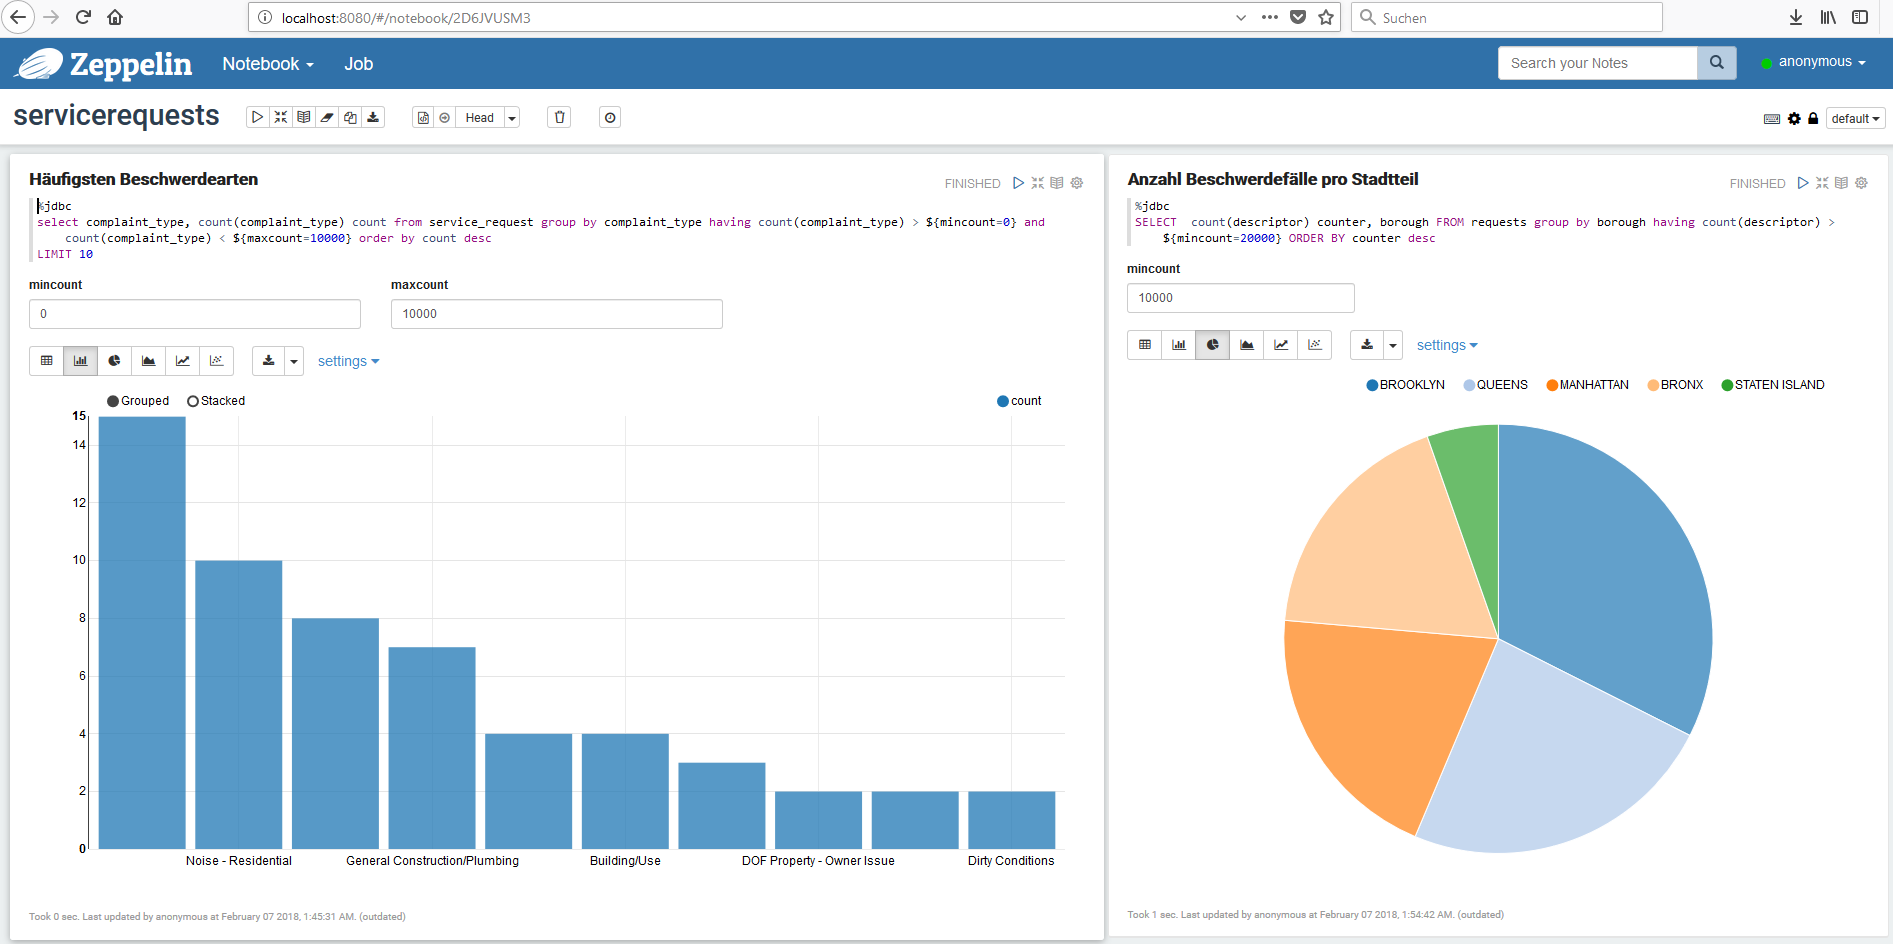
\includegraphics[width=\linewidth]{dualComplainChart.png}
	\caption[Ausschnitt des Notebooks]{Ausschnitt des Notebooks}
	\label{fig:zeppelin1}
\end{figure}
\begin{figure}[h] 
	\centering
	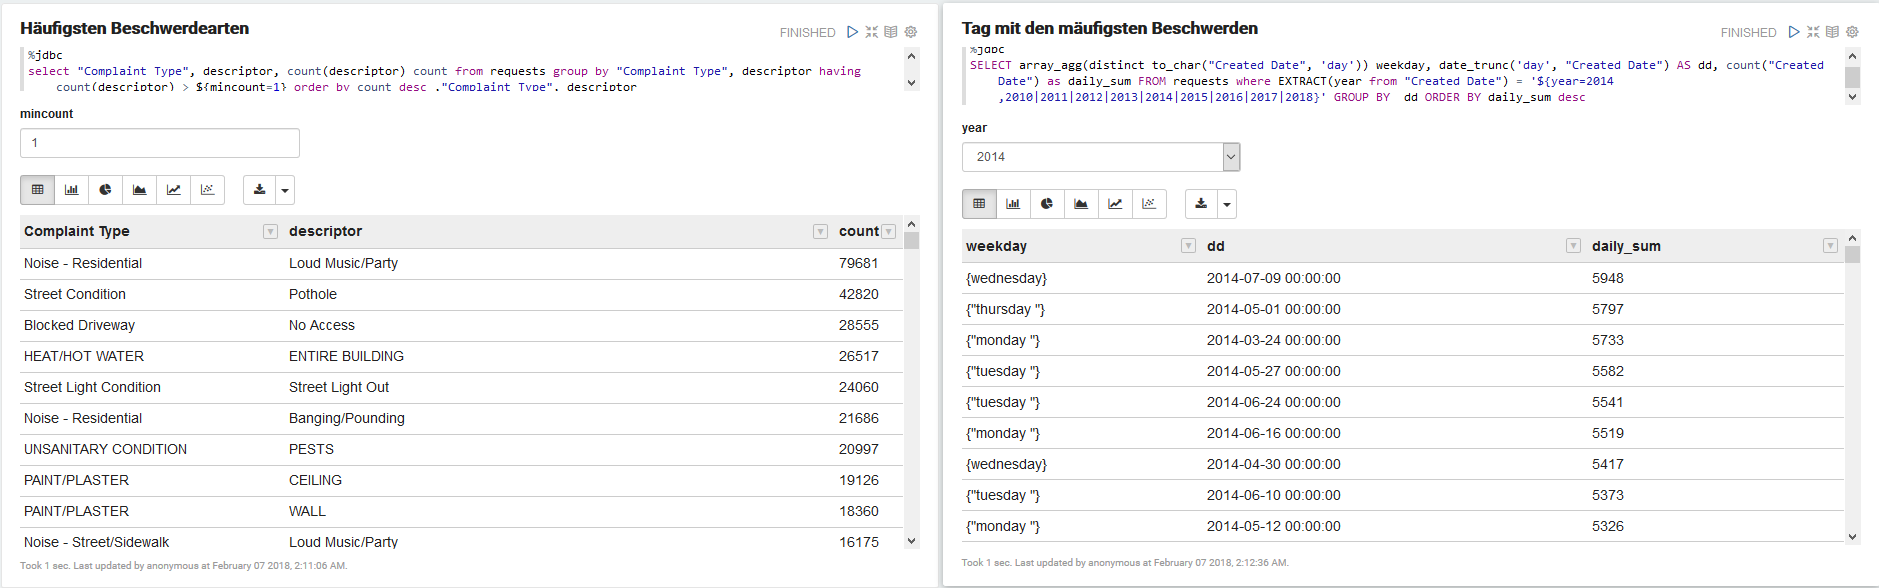
\includegraphics[width=\linewidth]{dualComplainDaychart.png}
	\caption[Ausschnitt des Notebooks]{Ausschnitt des Notebooks}
	\label{fig:zeppelin2}
\end{figure}
\begin{figure}[h] 
	\centering
	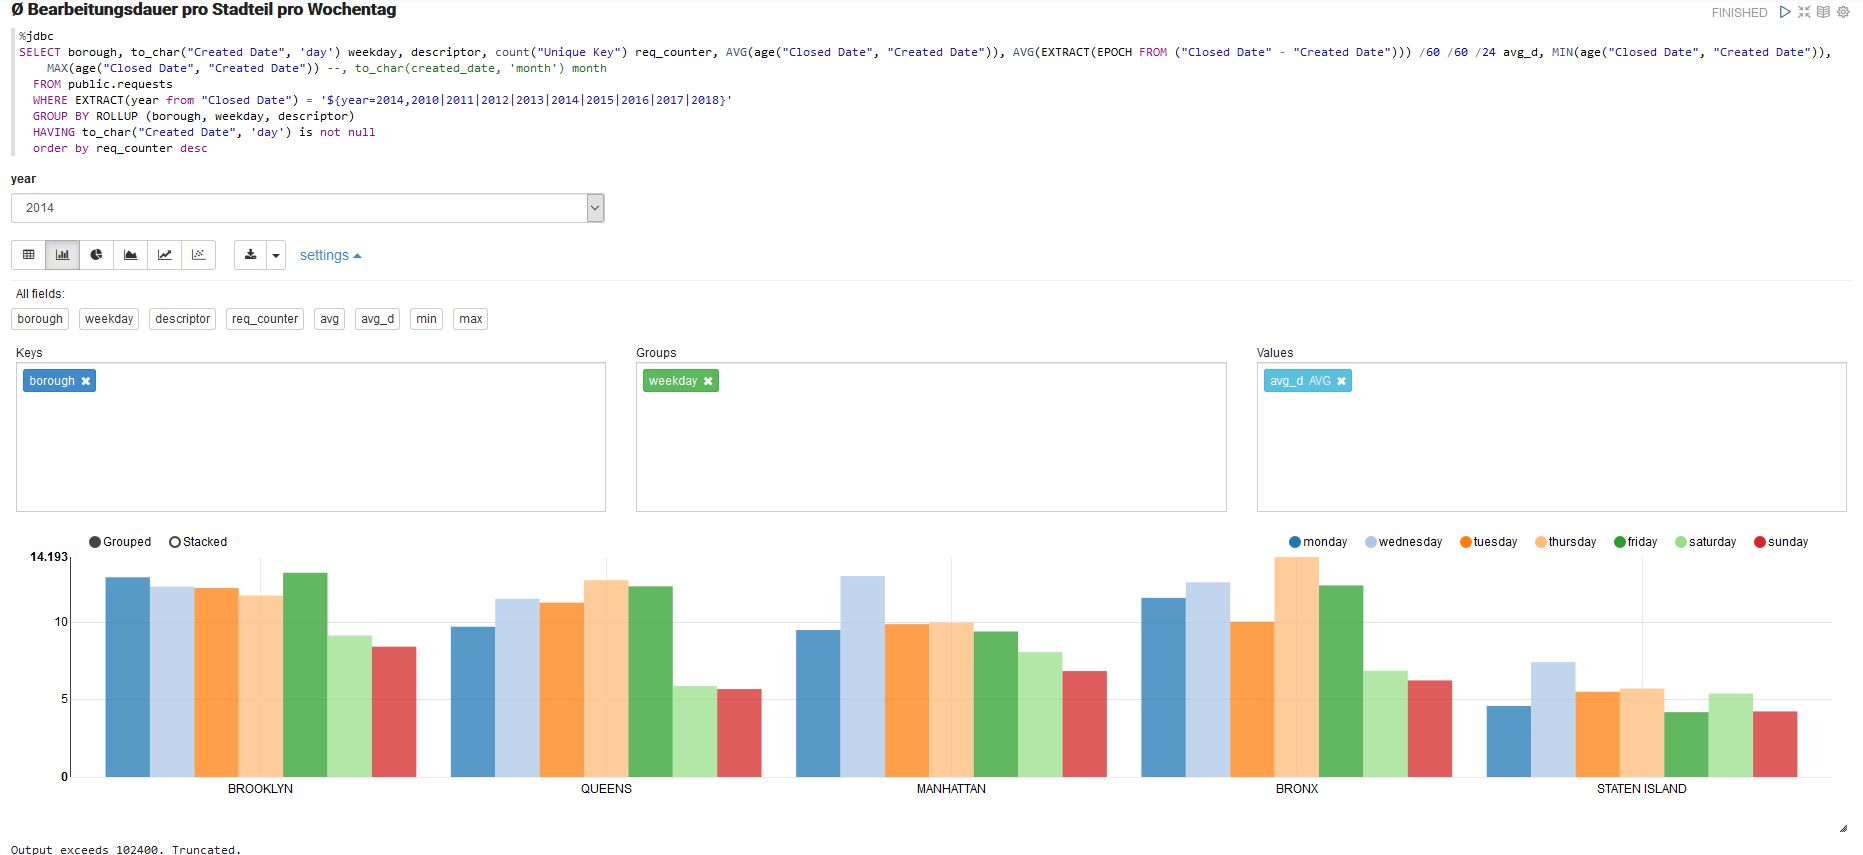
\includegraphics[width=\linewidth]{comByRegion.png}
	\caption[Ausschnitt des Notebooks]{Ausschnitt des Notebooks}
	\label{fig:zeppelin3}
\end{figure}



\subsection{Data Retrieval mit Jupyter}
Das Jupyter Notebook bietet die Möglichkeit mit \textit{Magic-Commands} direkt aus dem Notebook heraus
eine Verbindung mit der Datenbank aufzubauen und \ac{SQL} Statements abzusetzen.
Einfache Tabellen werden direkt in Jupyter visualisiert wohingegen komplexere Visualisierungen wie \zb{}
Balkendiagramme oder Geo Plots mit Python Bibliotheken dargestellt werden müssen.
Für die Darstellung in Jupyter werden sog. \textit{Widgets} installiert und aktiviert.


Folgende Python Bibliotheken wurden installiert um \ac{SQL} Statements in Jupyter ausführen und visualisieren zu können.
\begin{itemize}
  \item ipython-sql
  \item sqlalchemy (wird von ipython-sql benötigt)
  \item bokeh
  \item gmaps
\end{itemize}

Mit \code{ipython-sql} werden \ac{SQL} \textit{Magic-Command} in Jupyter aktiviert.
\code{ipython-sql} nutzt \code{sqlalchemy} um sich mit der Datenbank zu verbinden.
Ein abgesetztes \ac{SQL} Statement lässt sich entweder direkt in Jupyter ausgeben
oder einer beliebigen Variable zuordnen die dann weiterverarbeitet werden kann.


 \code{bokeh} ist eine mächtige Python Bibliothek um viele Arten der Visualisierung umzusetzen
 wie \zb{} Balkendiagramme, Scatter Plots, Geo Maps oder Zeitreihen.


 Die Visualisierung von Geo Daten erfolgt mit der Bibliothek \code{gmaps}.
 Diese greift auf die Karten von Google Maps zu erlaubt es die Geo Daten in einem Layer über einen
 beliebigen Kartenausschnitt zu legen.
 Der Vorteil von \code{gmaps} gegenüber \code{bokeh} ist
 zum einen die Nutzung des Kartenmaterials von Google aber auch die interaktive Nutzung
 des Kartenauschnitts mit \zb{} StreetView.


Folgende Fragestellungen wurden im Rahmen von Data Retrieval beantwortet.

\begin{enumerate}
  \item Zeige alle Beschwerdetypen die häufiger als 400 aber seltener als 8000 Mal gemeldet wurden?
  \item Wie lautet die Beschreibung der häufig vorkommenden Service Requests?
  \item An welchen Orten von New York City wurden Service Request vom Typ 'Noise - Residential' abgesetzt?
  \item Wieviele Service Requests sind im Jahr 2017 eingegangen? Gruppiert nach Tag und Sortiert nach dem Erstellungsdatum.
\end{enumerate}

Nachfolgender Abschnitt listet die \ac{SQL} Statements zu jeder Fragestellung sowie ein dazugehöriges Beispiel.


\textbf{zu 1.}
\newline
\sql{SELECT complaint\_type, COUNT(complaint\_type) FROM service\_request GROUP BY complaint\_type HAVING COUNT(complaint\_type) > 400 AND COUNT(complaint\_type) < 8000}

\bildhochkant{select_1.png}{Tabelle mit allen Beschwerdetypen}{srt}{eigene Darstellung}

\textbf{zu 2.}
\newline
\sql{SELECT descriptor, COUNT(descriptor) FROM service\_request  WHERE descriptor IS NOT NULL GROUP BY descriptor ORDER BY count DESC}

\bild{select_2.png}{Auszug aus den meisten Service Requests}{toprequests}{eigene Darstellung}{0.75}

\textbf{zu 3.}
\newline
\sql{SELECT longitude, latitude FROM service\_request WHERE complaint\_type = 'Noise - Residential' and latitude IS NOT NULL and longitude IS NOT NULL}

\bild{select_3.png}{Heatmap der Lärmquellen in New York}{rnnyc}{eigene Darstellung}{0.75}

\textbf{zu 4.}
\newline
\sql{SELECT date\_trunc('day', created\_date) AS dd, COUNT(created\_date) as daily\_sum FROM service\_request where EXTRACT(year from created\_date) = '2017' GROUP BY dd ORDER BY date\_trunc('day', created\_date)}

\bild{select_4.png}{Timeline aller Service Requests in 2017}{sr2017}{eigene Darstellung}{0.75}



\chapter{Inbetriebnahme}
\label{chap:betrieb}
In diesem Kapitel werden die einzelnen Schritte beschrieben, welche durchgeführt werden müssen um den Prototyp ausführen zu können.

\textbf{Hinweis:}
\newline
Hierbei handelt es sich lediglich um eine grob-granulare Beschreibung der Inbetriebnahme des Prototypen.
Weitere Details zur Installation und Nutzung können den Quellen entnommen werden.

\section{Voraussetzung \& Infrastruktur}
\subsection{Installation}
Folgende Komponente \underline{müssen}  installiert und lauffähig sein:
\begin{itemize}
  \item Apache Kafka und Apache Zookeeper
  %\item Apache Kafka Topic mit dem Namen \textitbf{ServiceRequests} erstellen\autocite{KafkaTopic}
  \item PostgreSQL
\end{itemize}


Je nachdem welche Technologie man für die Consumer, Producer und Auswertung verwenden möchte ergeben sich folgende zwei \underline{alternative} Technologiestacks:
\setlength{\columnseprule}{1pt}
\def\columnseprulecolor{\color{black}}
\begin{multicols}{2}
	\begin{itemize}
		\item Python 2
		\item pip
		\item Jupyter
	\end{itemize}
\columnbreak
	\begin{itemize}
		\item JDK 1.8
		\item Maven
		\item Apache Zeppelin
	\end{itemize}
\end{multicols}

\section{Infrastruktur Setup \& Konfiguration}
\begin{enumerate}
	\item Projekt aus Git Repository\footnote{\hyperref[hier]{https://github.com/johannesweber/BDBA\_DataEngineering.git}} auschecken
	\item Apache Zookeeper starten und initialisieren
	\item Apache Kafka starten und initialisieren
	\item Kafka Topic anlegen
	\item PostgreSQL Datenbankschema initialisieren\footnote{DDL Skripte um das Datenbankschema in PostgreSQL aufzubauen befinden sich im Ordner /db}
\end{enumerate}

\section{Setup und Starten des Python Prototypen }

\begin{enumerate}
  \item Python Bibliotheken installieren
  \begin{itemize}
    \item \shellcmd{pip install sodapy}
    \item \shellcmd{pip install kafka-python}
    \item \shellcmd{pip install psycopg2}
    \item \shellcmd{pip install sqlalchemy}
    \item \shellcmd{pip install jupyter}
    \item \shellcmd{pip install bokeh}
    \item \shellcmd{pip install ipython-sql}
    \item \shellcmd{pip install gmaps}
  \end{itemize}
  \item \texttt{gmaps} Widget für Jupyter aktivieren
  \begin{itemize}
    \item \shellcmd{jupyter nbextension enable --py --sys-prefix widgetsnbextension}
    \item \shellcmd{jupyter nbextension enable --py --sys-prefix gmaps}
  \end{itemize}
  \item Google Maps \ac{API} Key erstellen um die Google Maps Visualisierungen nutzen zu können\footnote{Eine Anleitung zum Erzeugen eines \ac{API} Keys gibt es \hyperref[hier]{http://jupyter-gmaps.readthedocs.io/en/latest/authentication.html}}
  \item Applikation Token für die \ac{SODA} \ac{API} beziehen\autocite{AppToken}
  \item Python Konfigurationsdatei \texttt{/python/config.py} pflegen
  \item Python Consumer und Producer starten via \texttt{/python/main.py}
  \item Jupyter starten und vorkonfiguriertes Notebook BDBA/DataEngineering.ipynb laden
\end{enumerate}

\section{Setup und Starten des Java Prototypen }

\begin{enumerate}
	\item CSV Datei von \hyperref[https://data.cityofnewyork.us/Social-Services/311-Service-Requests-from-2010-to-Present/erm2-nwe9]{https://data.cityofnewyork.us/Social-Services/311-Service-Requests-from-2010-to-Present/erm2-nwe9} runterladen und lokal speichern (ca. 11GB).
	\item Java Projekt mit Maven \shellcmd{mvn clean install} bauen.
	\item Konfiguration \texttt{/java/src/main/resources/kafka\_config.properties} pflegen.
	\item Python Consumer und Producer starten via \texttt{com.srh.bdba.dataengineering.Main}. Beim Aufruf der \texttt{Main()} muss man den Pfad zur CSV Datei angeben.
	\item Apache Zeppelin starten und Datenbankverbindung sowie JDBC Treiber im PSQL Interpreter pflegen\footnote{TODO sceenshot im Anhang}.
	\item Vorkonfiguriertes Notebook BDBA/zeppelin\_servicerequests\_notebook.json laden und Abfragen ausführen.
\end{enumerate}

\chapter{Zusammenfassung \& Fazit}
\label{chap:fazit}

% fazit in die loesung packen? Fazit = Fazit zum Vergleich der Tools und der eingesetzetn Architektur
% architektur gut weil
% kafka hat ALLE Daten
% postgres nur daten mit sinn!
% macht kein sinn auf unserer architektur aber definitv big data
% Obwohl unsere konkrete Implementierung
% kafka connectoren wäre besser
% jupyter vs. zeppelin feature vergleich
% java vs. python vs. kafka stream vs. kafka connect
\subsubsection{Gesamtarchitektur}

Apache Kafka wird dazu verwendet um alle empfangenen Datensätze ungeachtet ihres Inhaltes in einem Topic zu speichern.
Für dieses Projekt relevante Informationen wurden dann in die PostgreSQL Datenbank übertragen und konnten dann von dort mittels Apache Zeppelin und Jupyter ausgewertet werden.

Aufgrund der limitierten Größe unseres Datensatzes und der Rechenleistung des verfügbaren Equipments in unserem Projekt
hätte auf Apache Kafka verzichtet werden können, sodass die Daten direkt aus der \ac{API} in die Datenbank geschrieben werden
ohne den \glqq Umweg\grqq{} über Apache Kafka.\\
Jedoch ist in einem realen Szenario dieser Weg über Apache Kafka keineswegs falsch.\\
Dieser Ansatz ermöglicht es in der Datenbank nur diejenigen Daten vorzuhalten, die für die Beantwortung einer konfirmatorischen Frage notwendig sind und trägt damit zu einer besseren Performance bei. Zudem ist es leichter die Ausfallsicherheit und damit Verfügbarkeit der Daten in einem Kafka Cluster zu erreichen als in einem relationalen DB Cluster.
Darüber hinaus kann mit der Verwendung von Kafka Streams das original Topic gezielter angepasst und erneut wiedergeben werden.

Kafka Streams ist eine Klient Bibliothek zur Verfügung gestellt von Confluent.
Mit dieser Bibliothek können Anwendungen und Microservices erstellt werden, die eingehende Daten eines Topics
auslesen, weiterverarbeiten und in zweites, vor allem separates, Topic schreiben.
Kafka Streams bieten, wie alle Komponenten des Kafka Ökosystems, den Vorteil, dass sie untereinander hoch integriert,
hoch skalierbar und fehlertolerant sind.\\
Die dafür empfohlenen Programmiersprache von Confluent ist Java,
jedoch gibt es auch Implementierungen für andere Sprachen wie \zb{} Python.\autocite{KafkaStreams}

\subsubsection{Consumer \& Producer Implementierungen}
Beim Vergleich der beiden Implementierung für jeweils Kafka Producer und Kafka Consumer fällt auf, dass die Java Implementierung eher mit low-level APIs operiert und damit mehr Aufwand für Konfiguration und Konvertierung von Daten anfällt, wohingegen Python durch Verwendung von Frameworks, die Komplexität stärker abstrahieren, und schlankerer Syntax mit deutlich weniger Codezeilen auskommt. Somit stellt Python für einen PoC bzw. Prototypen die schnellere Alternative da, wobei Java und sein feinerer Detailgrad eher in komplexeren Umgebungen seine Stärken ausspielen kann.\newline
Aufgrund dessen, dass die Komplexität unserer Consumer und Producer insgesamt gering ist, da keine inhaltliche Transformation der Daten stattfindet, empfiehlt es sich für den produktiven Betrieb eher Kafka Connector zu evaluieren.\\
Kafka Connector sind ein  Teil der Confluent-Plattform und bilden Connectoren zu gängigen Datenquellen und -senken. Dabei setzen sie auf deklarative Konfiguration anstatt individuelle und imperative Programmskripte. Zudem bieten sie Fehlertoleranz und bessere Skalierbarkeit als einzelne Consumer bzw. Producer Skripte.

\subsubsection{Analysewerkzeuge}
Obwohl Apache Zeppelin im Mai 2016 den Incubator Status verlies macht es im allgemeinen einen noch sehr unreifen und unfertigen Eindruck,
was bei Versionsnummer 0.7 nichts überraschendes ist.
Bemerkbar macht sich dies vor allem bei der Installation und Setup insbesondere unter Windows.
So glückte der Start von Zeppelin auf nur 1 von 3 Windows PCs.
Des weiteren stürze der JDBC Interpreter während des Betriebs mehrfach aus unerfindlichen Gründen ab, was nur durch einen Neustart behoben werden konnte.
Zudem bietet Zeppelin 0.7 leider nur sehr rudimentäre Charting-Funktionalitäten.
Zwar gibt es eine Vielzahl an externen Plug-Ins die via Zeppelins Erweiterungsframework \textit{Helium} eingebunden werden können und erweiterte Diagrammtypen\footnote{z.B. Kartendienste und  Heatmaps, siehe \href{https://zeppelin.apache.org/helium_packages.html}{https://zeppelin.apache.org/helium\_packages.html} } bereitstellen, doch setzen diese Plug-Ins oft Zeppelin Version 0.8-\textit{SNAPSHOT} voraus. Diese Entwicklungsversion kann man nur per Sourcecode beziehen und selber kompilieren bzw. bauen.
Das klappte sogar nach mehreren Versuchen, jedoch ließ sich das fertige \textit{binary} nicht starten.\newline
Letztlich lässt sich zusammenfassen, dass die Konzepte hinter Apache Zeppelin gut sind, die konkrete Implementierung jedoch noch nicht ausgereift ist.

Die Installation und Erstkonfiguration mit Jupyter unter Windows ist in wenigen Minuten erledigt.
Sobald Jupyter und die \text{Magic-Commands} mit dem Paketmanager \textit{pip} installiert wurden können
schon erste \ac{SQL} Statements abgesetzt werden.\\
Resultate eines \ac{SQL} Statements werden grafisch als Tabelle dargestellt.
Für jegliche Art von Visualisierung die darüber hinaus geht müssen separate Bibliotheken installiert werden
über die dann die Visualisierung erfolgt.
Zusätzlich müssen \textit{Widgets} installiert und aktiviert werden wenn die Grafik integriert in Jupyter angezeigt werden soll.\\
Auch hier gibt es Einschränkungen: Falls kein Widget für die aktuell genutzte Bibliothek zur Verfügung steht kann nur die Anzeigemöglichkeiten der Bibliothek genutzt werden.\\
Das dynamische Ändern eines \ac{SQL} Statements mit einem Textfeld - so wie es in Apache Zeppelin erfolgen kann - benötigt ihn Jupyter zwar zusätzlichen Implmentierungsaufwand kann aber letztlich genauso wie in Apache Zeppelin erfolgen.\\
Die \textit{Magic-Commands} sind sowohl in Apache Zeppelin als auch Jupyter eine sehr gute Möglichkeit um kleine Code Snippets mit \code{\ac{SQL}} oder \code{R} zu Prototypen ohne tief in die Programmierung einzusteigen.
Alles darüber hinaus wie komplexe Visualiserungen oder Manipulation der Ergebnisse erfordert die Nutzung von weiteren Bibliotheken und
Visualisierung können nur bedingt in Apache Zeppelin und Jupyter angezeigt werden.

In unserem Projekt haben wir die Erkenntnis gewonnen, dass die virtuellen Notebooks für schnelles Prototyping sehr gut geeignet sind.
Will man aber das Notebook so anpassen, dass \zb{} dynamisch Daten von einer externen Datenquelle abgerufen werden
und sich die genutztes Charts kontinuierlich anpassen - Stichwort Real-Time Monitoring - dann ist wesentlich mehr Aufwand nötig und man stellt sich die
Frage ob die virtuellen Notebooks dafür noch geeignet sind und nicht für dieses Szenario ein anderes oder weitere Tools benötigt werden. In diesem Umfeld sind vor allem die Open Source Werkzeuge Kibana von Elastic und Grafana zu nennen.\\
Die Erstellung eines Monitoring-Dashboards mit Echtzeit Metriken in Kombination mit einem Notebook für explorative Analytik birgt weitere interessante Ansätze und Überlegungen die
jedoch, mit Hinblick auf das Projektziel, nicht weiter verfolgt wurden.


% ------------------------------------------------------------------

\label{lastpage}

% Neue Seite
\cleardoublepage
\phantomsection

% Backmatter mit normalem Zeilenabstand setzen
\backmatter
\singlespacing

% Römische Ziffern für die "Back-Matter", fortlaufend mit frontmatter
\pagenumbering{roman}
\setcounter{page}{\value{frontmatterpage}}

% Abkürzungsverzeichnis
\chapter{Abkürzungsverzeichnis}

\begin{acronym}
\acro{ITIL}[ITIL\textsuperscript{\textregistered}]{IT Infrastructure Library}
\acro{ITSM}{IT Servicemanagement}
\end{acronym}


% Abbildungsverzeichnis erzeugen
\cleardoublepage
\phantomsection
\addcontentsline{toc}{chapter}{Abbildungsverzeichnis}
\listoffigures

\end{document}
